% TEMPLATE for Usenix papers, specifically to meet requirements of
%  USENIX '05
% originally a template for producing IEEE-format articles using LaTeX.
%   written by Matthew Ward, CS Department, Worcester Polytechnic Institute.
% adapted by David Beazley for his excellent SWIG paper in Proceedings,
%   Tcl 96
% turned into a smartass generic template by De Clarke, with thanks to
%   both the above pioneers
% use at your own risk.  Complaints to /dev/null.
% make it two column with no page numbering, default is 10 point

% Munged by Fred Douglis <douglis@research.att.com> 10/97 to separate
% the .sty file from the LaTeX source template, so that people can
% more easily include the .sty file into an existing document.  Also
% changed to more closely follow the style guidelines as represented
% by the Word sample file. 

% Note that since 2010, USENIX does not require endnotes. If you want
% foot of page notes, don't include the endnotes package in the 
% usepackage command, below.

% This version uses the latex2e styles, not the very ancient 2.09 stuff.

% Updated July 2018: Text block size changed from 6.5" to 7"

\documentclass[letterpaper,twocolumn,10pt]{article}
\usepackage{usenix2019,epsfig,endnotes,algpseudocode,algorithm}
\begin{document}

%don't want date printed
\date{}

%make title bold and 14 pt font (Latex default is non-bold, 16 pt)
\title{\Large \bf Hacking Electronic Internet Connected Shifters }

%for single author (just remove % characters)
\author{
  {\rm Thomas Hansen}\\
  UW Madison
  \and
  {\rm Tolga Beser}\\
  UW Madison
  \and
  {\rm Chang-Yen Tseng}\\
  UW Madison
  % copy the following lines to add more authors
  % \and
  % {\rm Name}\\
  %Name Institution
} % end author

\maketitle

% Use the following at camera-ready time to suppress page numbers.
% Comment it out when you first submit the paper for review.
\thispagestyle{empty}


\subsection*{Abstract}


\section{Introduction}

% A paragraph of text goes here.  Lots of text.  Plenty of interesting text. \\

% More fascinating text. Features\endnote{Remember to use endnotes, not footnotes!} galore, plethora of promises.\\

Cyclists has seen the emergence of wireless shifting technologies over the past few years. While the technology existed as far back as the 1990s, adoption has accelerated in recent years, especially for high-end bikes. As we see the technology improve, these shifters have become faster and more precise than mechanical shifting, accelerating their adoption among riders.

The wireless shifters use an assortment of communication technologies known as Personal Area Networks (PAN’s) such as Bluetooth. The use of these technologies opens the once closed off bicycle to security vulnerabilities. If an attacker can trigger extraneous shifts the cyclist can be thrown off their bike causing personal injury and the potential for even larger accidents (cyclists in pro races are tightly packed causing crashes to spread quickly). While security research focused on these electronic shifters is sparse there exists a plethora of work exploring security for various Personal Area Network enabled devices. A subset of wireless shifters utilizes Bluetooth as a communication protocol which has been shown to have security flaws in several implementations. One of the wireless shifting devices that we would like to examine is the SRAM eTAP system which utilizes their novel Airea Personal Area Network protocol which allows their components to communicate from up to a hundred meters away. This large distance could allow an attacker to communicate with their components from an unobservable location.

\section{Related Work}

There has been a lot of work into researching how to break wireless networks on embedded electronic devices, especially those where security is not the strong suit. Many simply use replay attacks and exploit design flaws with device authentication~\cite{Halperin}. Other papers look broadly on the state of wireless security, and analyse methods surrounding IoT devices and wireless communication methods~\cite{Choi}~\cite{Radek}.

We attempted to take many of these findings and bring them to the electronic shifting space, and see what sorts of vulnerabilities we could find. To the best of our knowledge, no comprehensive research yet has existed on the security wireless shifters for bikes. We studied the Archer Components D1X, SRAM eTap, and Shimano Di2 for vulnerabilities.

\section{Potential Impact}

Electronic shifters in bikes have become extremely popular among high-end bikes. Tadej Pogačar, the overall winner of the 2021 and 2020 tour won using a Campagnolo EPS shifter. Egan Bernal, the 2019 winner, won riding a Pinarello that used Shimano Dura Ace Di2 shifters~\cite{GCNTech}. Furthermore high-end bikes, such as the Trek Madone 9, are sold by defualt with electronic shifters.

Competitions furthermore have high stakes. The Tour de France prize pool is 3.6 million AU, and many millions stand to be gained from partnerships and sponsors. Anyone who's able to impact a race in their favor may realize substantial financial gain, and we only expect the potential professional impact to expand with time.

Lastly is the impact on line. Biking is a sport where even more casual riders will go for hours, and being able to disable a bike and strand someone somewhere can make them more vulnerable or otherwise threaten their wellbeing. It's because of all of these reasons we think the security of electronic shifters is an important topic that deserves research.

\subsection{Contributions}

Our major contribution to the field was bringing proper security testing to electronic sifters in the biking industry. These devices have become increasingly popular among professionals and performance cyclists, and there's no real analysis of which devices provide the best, if any, security to the biker.

Some devices, like the STRAM eTap, claim

\subsection{Common Attacks Against IoT Devices}

The security of IoT Devices is well documented and various devices have been studied in recent years. [cite papers here] Because the research body is so vast we will derive a few common attack vectors. The attack vectors that we will outline are Replay Attacks[cite], Denial of Service[cite], and Man in the Middle Attacks[cite].
\\\\
(1) Replay Attacks are conducted by recording communication signals between IoT Devices and replaying them. Without a dynamic key(not sure if this wording is right) these false signals will be non-discernible from the legitimate commands. [cite] \\
(2) Denial of Service(DDOS) attacks have been shown to be effective against a variety of IoT devices. Lack of processing power among small IoT devices compounds their risks to such attacks. [cite] \\
(3) Man in The Middle(MITM) attacks intercept communications from IoT devices and proceed to act as the expected receiver/communicator.[cite]\\


\subsection{Research in wireless attacks against other vehicles}

The ushering in of new technology to bicycles is reminiscent of the automotive industries push towards intelligent systems. These changes, however, come with their own security issues which was highlighted when Chrysler recalled 1.4 million vehicles due to a remote hacking vulnerability that let adversaries control the vehicle and even cut the brakes ~\cite{ChryslerRecall}. Remote vehicle hacking has been demonstrated across multiple manufacturers (Tesla, BMW, Chrysler) ~\cite{Tesla}~\cite{BMW}~\cite{Chrysler}.  and research into the security of such systems is now commonplace [cite survey]. Systems utilized by intelligent vehicles such as vehicular ad hoc networks~\cite{ dibaei2019overview} (VAHN) enabling vehicle to vehicle communication have been studied and found to pose security risks~\cite{ SAKIZ201733}. With the rise of intelligent/wireless bicycle components the need to assess a security landscape of such components becomes paramount as seen by the changes in the automotive industry. 

% \section{Threat Model}

\section{Devices}
\subsection{Archer Components D1X}

The Archer D1X~\cite{Archer} is a modular electronic shifting system that can be integrated into a wide array of derailleur-shifting groupsets. While the other two components groups that we study come with custom derailleurs that are wirelessly enabled, the D1X focuses on integrating into existing systems. It is installed near the derailleur with the shifting cables routing through it. This allows the D1X to change the tensions of the shifting cables and triggering gear changes. The electronic shifting box is connected to the hand shifters through Bluetooth allowing the user to send shifting signals. Of note, the D1X is the only component that we will study that utilizes the Bluetooth protocol for communication between the shifter and shifting box.

The setup for the D1X is largely influenced by the Bluetooth protocol. On first use, the hand shifter needs to pair with the users phone using the mobile application~\cite{ArcherApp}. After the user has paired the shifter they need to initiate a remote pairing through the application allowing the shifting box to pair with the hand shifter. This is a one time pairing process, subsequent uses do not require these steps. The user can connect to the shifting box through the Archer mobile application. This is done by turning on the shifting box and going to the Archer application to pair. Through the application the user can set shifting profiles allowing them to dictate specific gears that should be changed upon a shifting command. 

\subsection{Shimano Di2}

The Shimano Di2 (ultegra) model shifters are a high performance bike part that's regularly used by professional cyclists and consumers. It's an electronic wired component, with an added wireless unit, the EW-WU111, which can be used to connect to a phone app over bluetooth. The wireless unit sits inside the frame, and can be added or removed without change to the shifters functionality.

\begin{figure}[ht]
\begin{center}
\centering
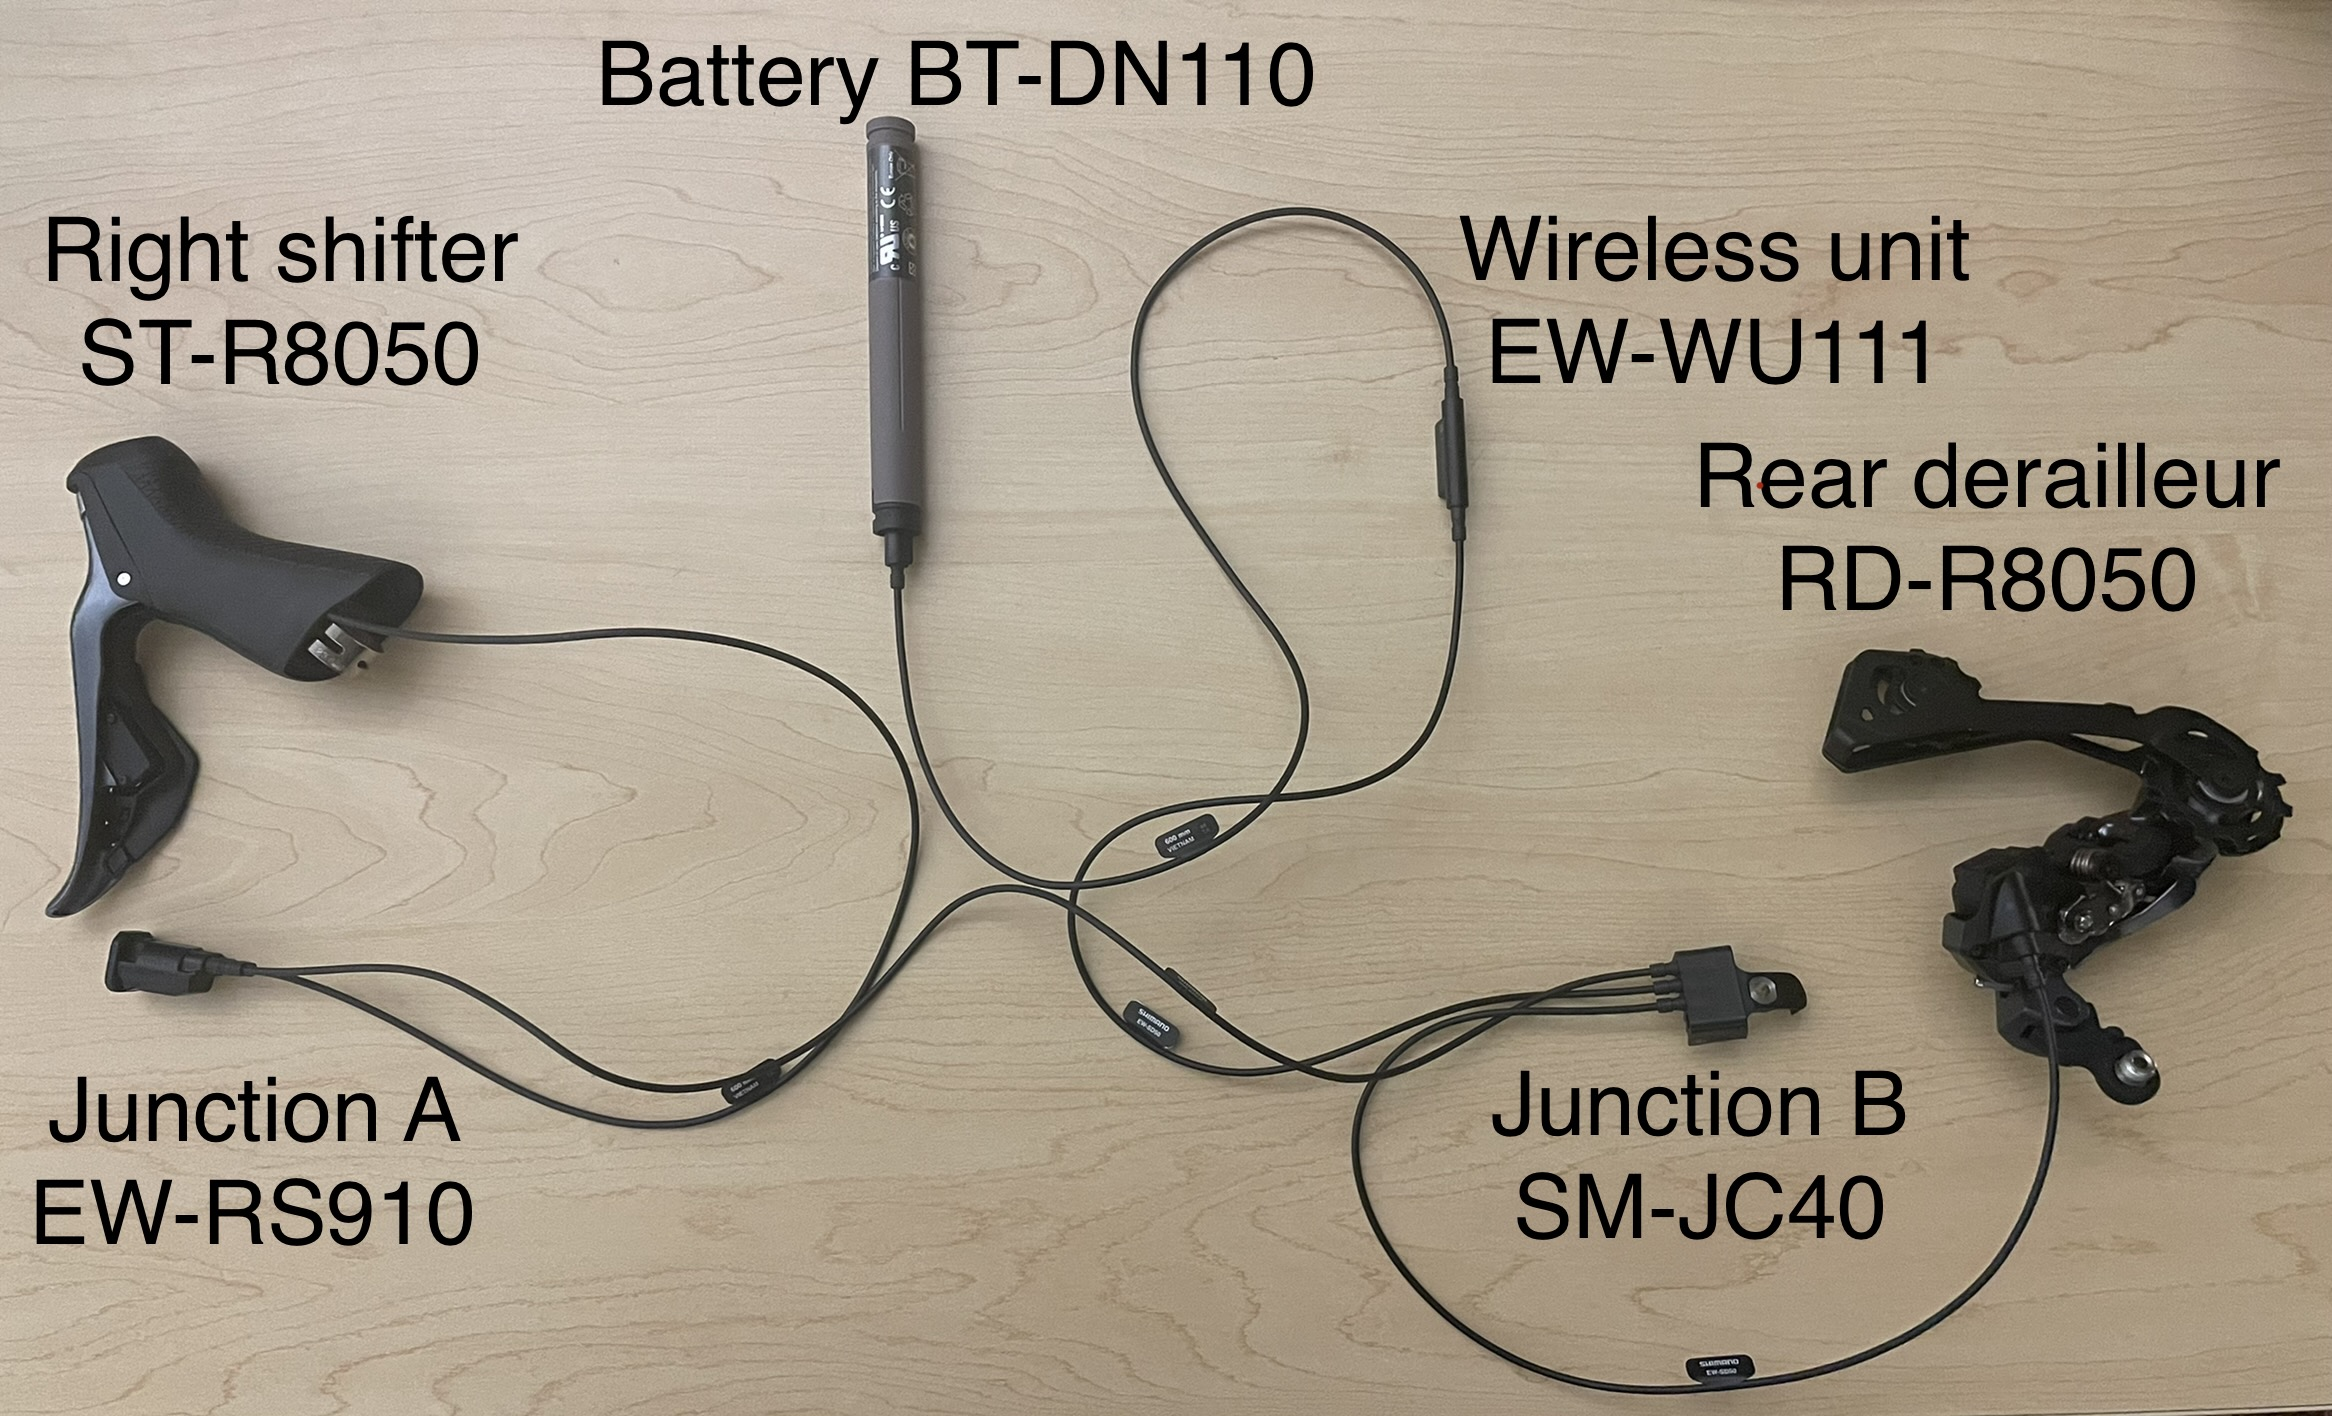
\includegraphics[width=0.4\textwidth]{images/IMG_5264_Di2.jpg}
\label{fig:Di2Setup}
\end{center}
\caption{The battery sits inside the seat post while the rear derailleur sits on the back wheel. The junctions sit at mount points in the frame/handlebar, and the wireless unit floats freely in the frame}
\end{figure}

The phone app, E-TUBE, seems to be more robust than the archer components model. Once connected to a phone, the Di2 system will no longer shift using the hand shifter and other phone users can't boot the initial phone user off without the initial phone user disconnecting first. It also disallows users from using the device while connected to bluetooth, so although this could be used to deny service it will primarily allow bikers to know immediately when an attacker connects to their device instead of allowing an attacker to sign on and adjust the shifter alignment using the default app. Most significantly, however, the Di2 system has the option for up to a 6 digit pin so long as the final pin isn't a 0, or 2.56E12 combinations. This pin automatically saves on the device once you enter it and is visible in plain text to anyone using the phone. A user who enters a wrong passkey on the phone app receives an error message and forces the user to restart the Di2 junction, and from what we can tell this is a feature of the junction (we tested on an EW-RS910 Junction A). Because of this, brute forcing your way in if the user has a passcode set is effectively impossible.

\subsection{SRAM Force eTap AXS}
The SRAM Force eTap AXS \cite{etap} is marketed toward professional, competitive bikers, and is price most premium out of all of our components. It works completely wirelessly like the Archer Components D1X, where there is no need for physical wire between the derailleur and the shifters. The SRAM is also the only one in our lineup that uses a proprietary protocol. The derailleur and the shifter communicate using the in-house AIREA protocol that operates within the 2.475Ghz frequency range. During a press event of this products, SRAM claims that  the protocol uses 128-bit rolling encryption and the system is "more secure than any cash machine".\cite{phillips2015SRAM} The system also provides Bluetooth for connecting to a smartphone and ANT+ to send information to a bicycle computer.

To set up the SRAM system, the biker will have to click a button on the derailleur to enter pairing mode and then click the buttons on both shifters consecutively to finish the pairing process. To connect to a mobile phone, the biker will start an app on their phone, select their SRAM system, and long-press a button on the derailleur to authorize. Note that the app provides ways to remap each shifter to different operations (gear up, gear down), but the user is not able to shift the gear directly in the app.




\section{Security Analysis}



\subsection{Threat Model \& Goal}
We want to protect the safety of the bikers with such electronic shifters as sudden shifting when unintended may cause massive harm. We assume a scenario where bikers are joined with some malicious actors in a large-scale biking competition. In this scenario, we assume the adversary has access to the type of shifter the victim is using. The adversary can also be in close proximity with the victim before or during the competition, as a result, they can send arbitrary radio signals to the victim. We further assume the adversary can have a very short period of physical access with the victim's bike before the competition, such as when the victim is not looking.

We define a successful attack as making a victim's bike shift to an unintended gear during competition. We will also define a successful attack as making a victims bike unable to respond to legitimate shifting commands during competition. We assume all competitors will do a quick test ride before the competition and don't consider denial of service before the competition as a successful attack since this does not introduce safety risks to the riders. For that reason, simple attacks such as cutting the victim's breaking cable or poking a hole in the victim's tire will be trivially easy to spot during the test ride and thus won't qualify as a successful attack.


\subsection{Bluetooth Pairing Weekness}

The Archer D1X groupset relies on the Bluetooth communication protocol for shifter/shifting-box communication along with communication with the mobile application. Once the shifting box is powered on anybody with the Archer mobile application can pair with it. There are no pairing authentication steps and this lack of validation means that those other than the legitimate owner can connect. Once an adversary has paired with the shifting box they can create custom gear-switch settings that would be harmful to the user. An adversary could swap the higher and lower gear switch buttons causing the cyclist to experience unexpected dangerous behavior. Gear setting changes made through the application are invisible to the cyclist and there is no mechanism of alerting the owner of such changes. The Bluetooth protocol only allows for one active device at a time meaning that only one device can be connected to the shifting box at a time. If an adversary were to pair with the shifting box through the Archer mobile application they would be able to block all hand shifter communication thus ceasing functionality.  

\subsection{SRAM Replay Attack}
From the public FCC data, we know that the SRAM system's operating frequency is around 2.475GHz with a bandwidth of 3MHz, therefore, we use an SDR and the Universal Radio Hacker software\cite{urh}  to analyze the signals between the shifters and the derailleur. We find out that every time the shifter is pressed, it will emit a signal continuously for about 1.2 seconds and we didn't observe any ACK-like signal from the derailleur. We further discover that recording a gearing event signal from a shifter and replaying it will cause the derailleur to act accordingly. However, the recorded packet will be invalid whenever the biker presses the same side of the shifter again. We suspect that each shifter has its own internal counter that the derailleur keep track of so it can invalidate all previous packet after receiving a new one.

However, the ability to replay the latest packet still opens up a way to attack the system. Based on the aforementioned vulnerability, we designed an algorithm specifically to attack an SRAM system during competition. We set up the SDR in a way that it will continuously switch between receiver and sender mode. During the receiver mode, the SDR will capture signals from the air and detect if it contains an SRAM gearing signal. If it does, it stores the new signal. Then it will send the saved signal (either the newly captured one or something stored before) to the air, causing the victim's bike to shift unintendedly. 

Since SRAM does not release their firmware let alone source code, we do not have a reliable way to detect whether a signal segment contains an SRAM shifting packet or not. Therefore, we use a simple SVM classifier to solve the problem. We prerecorded several SRAM gearing signal segments and trained the model along with white noise and signal from other 2.4Ghz devices. In the end, we can reach 100\% accuracy in a lab environment.

We setup the attack with a HackRF One SDR. Under the attack, when the victim shifts near the attacker, their derailleur will continuously shift to the highest or lowest, and even if the victim counter shift, they will find out that their system shift to the other extreme direction.
\begin{algorithm}
\caption{SRAM replay attack algorithm}\label{alg:cap}
\begin{algorithmic}[1]
  \State $saved \gets None$
  \While {$True$}
    \State Set up SDR in receiver mode
    \State $signal \gets$ get signal from SDR for 1 second
    \If{$signal\;match\;SRAM\;pattern$} 
        \State $saved \gets signal$
    \State Setup SDR in sender mode
    \State Send $saved$
    \EndIf 
  \EndWhile
  \end{algorithmic}
\end{algorithm}

\paragraph{Potential Optimization}
In the attack, if the victim happens to shift the same gear while the SDR is in sender mode, 
subsequent attacks will fail. However, there are possible ways to optimize this attack.
\begin{itemize}
  \item \textbf{Use two SDRs one for receiving and one for sending.} Clearly, in this setting, the attacker will be able to notice the victim's signal while they are sending their malicious signal. However, the attacker's receiver will now be interfered by their sender, and special care needs to be done to avoid confusion.
  \item \textbf{Trim the saved data.} During investigation, we found out that while the signal from the shifter lasted over 1 second, 50ms worth of data is enough to cause the derailleur to act. Therefore, it is possible that we can trim the data so that the SDR can send the data and be in sender mode for just a little amount if time, greatly reducing the chance of missing the victim's signal.
\end{itemize}


\section{Evaluation}

Our paper provides the first look at the security landscape of wireless bike shifting systems. We found that the communication protocol (Bluetooth vs AIREA) chosen vastly dictates the threat landscape. 

While Bluetooth protocols enable a wide array of integrations such as smartphone connections, they also require strict authentication enforcement. While the Shimano Di2 system enforced a pin requirement to connect via smartphone the Archer D1X didn’t and was completely open for adversaries to pair with. The Bluetooth protocol also limits active connections to one device at a time enabling adversaries to shut out legitimate users and in the case of the Archer D1X deny shifting capabilities. Once an adversary has paired with a component, they can change the various shifting settings without the user being notified. Due to the nature of shifting systems these changes won’t be noticed until the user attempts a shift creating a dangerous situation.

 As detailed in section 5.3 we found that the AIREA protocol implemented by the SRAM groupset was vulnerable to replay attacks. Though SRAM claims to utilize 128 bit rolling key encryption our attacks show that their systems are vulnerable. If utilized by an adversary during an event such as a cycling competition dangerous conditions could be created by even one rider losing balance due to unexpected shifting.


\section{Recommendations}



\section{Conclusions}




\section{Future Work}




  {\normalsize \bibliographystyle{acm}
  \bibliography{references}}

% \theendnotes

\end{document}


% Some embedded literal typset code might 
% look like the following :

% {\tt \small
% \begin{verbatim}
% int wrap_fact(ClientData clientData,
%               Tcl_Interp *interp,
%               int argc, char *argv[]) {
%     int result;
%     int arg0;
%     if (argc != 2) {
%         interp->result = "wrong # args";
%         return TCL_ERROR;
%     }
%     arg0 = atoi(argv[1]);
%     result = fact(arg0);
%     sprintf(interp->result,"%d",result);
%     return TCL_OK;
% }
% \end{verbatim}
% }

% you can also use the wonderful epsfig package...
% \begin{figure}[t]
% \begin{center}
% \begin{picture}(300,150)(0,200)
% \put(-15,-30){\special{psfile = images/piezospeaker.png hscale = 50 vscale = 50}}
% \end{picture}\\
% \end{center}
% \caption{Wonderful Flowchart}
% \end{figure}


% Example image
% \begin{figure}[ht]
% \begin{center}
% \centering
% \includegraphics[width=0.4\textwidth]{images/2msSig18.png}
%
% \label{fig:2msSignal}
% \end{center}
% \caption{Above is a signal generated with data, where each bit was transmitted over 2ms. This allowed us % to create high resolution bit maps where the bits are distinguishable from each other.}
% \end{figure}


% An example table if we need to display data
%
% \begin{table}[]
% \begin{tabular}{|l|l|r|}
% \hline
% \multicolumn{1}{|c|}{Action}        & Code   & Distance                      \\ \hline
% Right turn                          & 0b0001    &                               \\ \hline
% Left turn                           & 0b0010   &                               \\ \hline
% Change lane (right)                 & 0b0011   &                               \\ \hline
% Change lane (left)                  & 0b0100  &                               \\ \hline
% Merge (right)                       & 0b0101  &                               \\ \hline
% Merge (left)                        & 0b0110  &                               \\ \hline
% Offramp                             & 0b0111  & \multicolumn{1}{l|}{}         \\ \hline
% Temporarily change lanes (incident) & 0b1000 & \multicolumn{1}{l|}{}         \\ \hline
% Speed (speeding up)                 & 0b1001 & \multicolumn{1}{l|}{Not used} \\ \hline
% Speed (slowing down)                & 0b1010 & \multicolumn{1}{l|}{Not used} \\ \hline
% \end{tabular}
% \end{table}



% Itemized list example
%
% \begin{itemize}
% \item Example itemized list
% \item Item 2
% \end{itemize}


% Equation Example:
% 
% $$ f = f_{0} \frac{c \pm v_{r}}{c \pm v_{t}} $$


% Example Code
%
% {\tt \small
% \begin{verbatim}

% generateSignal(dataSet)
%     lf = rand_low_freq
%     hf = rand_low_freq + frequency_shift

%     bits = [1,0,1,0,0,1,dataSet]
%     freqs = ones(length(bits)) .* lf

%     % assign 1 bits to high frequency
%     for 1 = 1:length(bits)
%         if bits(i) == 1
%             freqs(i) = hf
%         end
%     end

%     % add frequencies to signal
%     for i = 1:length(packet)
%         t = 0:1/fs:bit_duration;
%         f = sin(2*pi*packet(i).*t + phase);

%         % update phase
%         phase = phase + 2*pi*packet(i)*bit_duration;

%         % add in next position
%         ff(start_leg:end_leg) = f;
%     end
% end
% \end{verbatim}}
